\section{Generative Adversarial Networks}
GAN (Generative Adversarial Networks), Ian Goodfellow ve Montreal Üniversitesi'nden diğer araştırmacılar tarafından 2014 yılında tanıtılmıştır. Üretken yapay zeka kümesine ait bir sinir ağıdır. İki sinir ağından oluşmaktadır. Generator (Üretici) ve Discriminator (Ayırıcı). Birbirlerine karşı yerleştirilirler. Generator, yeni örnekleri oluşturur. Discriminator, oluşturulan örneklerin gerçekliğini değerlendirir. Generator tarafından üretilen verileri gerçek ve sahte olarak sınıflandıran ikili bir sınıflandırıcıdır. Eğitim verileri buraya yüklenir. 

GAN'ın avantajları;
\begin{itemize}
	\item Gerçekçi Veri Üretimi
	\item Çeşitli Veri Üretimi
	\item Denetimsiz Öğrenme
	\item Görüntüden Görüntüye Çeviri
	\item Yaratıcı Uygulamalar
\end{itemize}

GAN'ın dezavantajları;
\begin{itemize}
	\item Eğitim İstikrarsızlığı
	\item Mod Daraltma
	\item Değerlendirme Metrikleri
	\item Hiperparametre Hassasiyeti
	\item Hesaplamalı Kaynaklar
\end{itemize}

Bazı GAN türleri:

\begin{enumerate}
    \item DCGAN (Deep Convolutional GAN)
    \item WGAN (Wasserstein GAN)
    \item SRGAN (Super Resolution GAN)
    \item pix2pix (Image to Image)
    \item CycleGAN (Cycle Generative)
    \item StackGAN (Stacked GAN)
    \item ProGAN (Progressive Growing)
    \item StyleGAN (Style-Based GAN)
    \item VQGAN (Vector Quantized)
    \item SGAN
    \item SAGAN
    \item AC-GAN
    \item GauGAN
    \item GFP-GAN
\end{enumerate}

\subsection{Çalışma Adımları}
Üretici rastgele gürültüden gelen bir girişi kullanarak veri setine benzeyen yeni örnekler üretir. Ayırıcı, bu örnekleri gerçek veya sahte olarak sınıflandırır. İki ağ da birbirine karşıdır. Üretici, ayırıcının sahte veri örneklerini gerçek olarak sınıflandırmasını engellemeye çalışırken, ayırıcı gerçek ve sahte örnekleri daha doğru bir şekilde ayırt etmeye çalışır. Bu sürekli rekabet ve geri besleme döngüsü sonucunda, hem üretici ağ daha gerçekçi veri örnekleri üretmeyi öğrenirken hem de ayırt edici ağ daha hassas bir şekilde gerçek ve sahte örnekleri ayırt etmeyi öğrenir.

Eğitim sırasında üretici ve ayırt edici ağ arasında bir denge sağlanmalıdır. Eğer üretici ağ çok iyi olursa ve ayırt edici ağ sahte verilerle gerçek verileri ayırt edemez hale gelirse model başarısız olabilir. 

\begin{figure}[h]
    \centering
    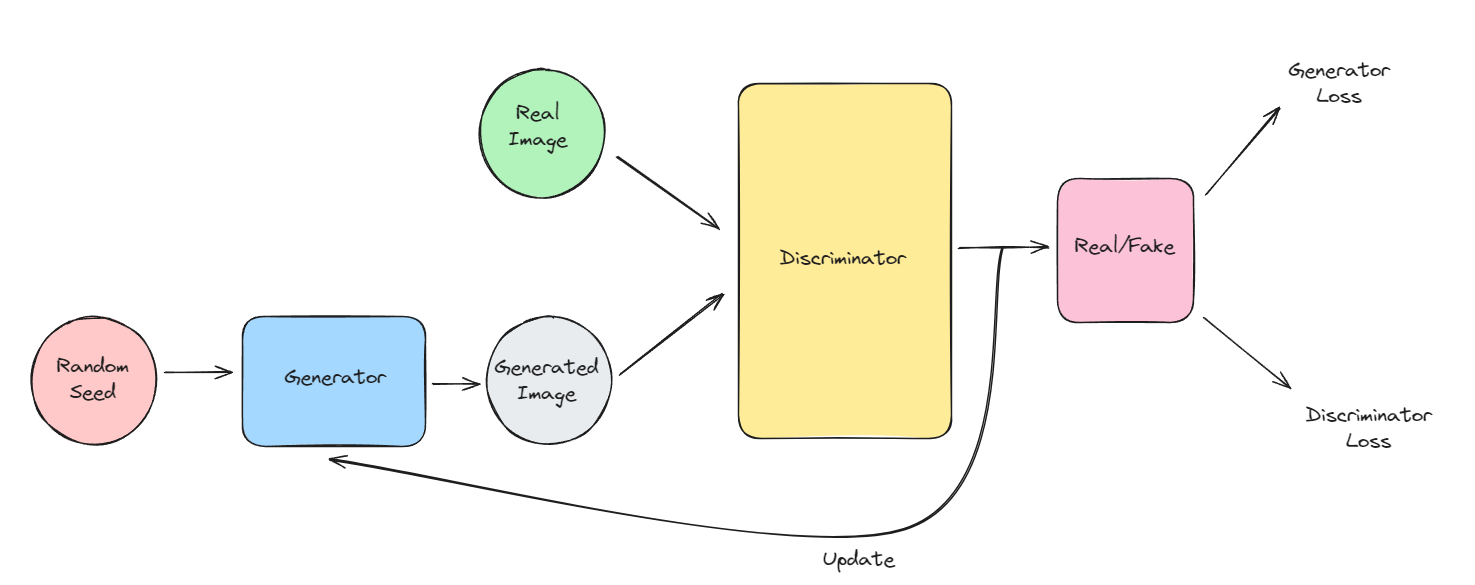
\includegraphics[width=1\textwidth]{images/gan_architecture.png}
    \caption{GAN mimarisi.}
    \label{fig:enter-label}
\end{figure}

\subsection{DCGAN (Deep Convolutional GAN)}
2015 yılında Radford ve diğerleri tarafından yayınlanmıştır. GAN'dan farkı FC (tam bağlantılı) katmanlar yerine CNN kullanır. DCGAN, özellikle resimlerin üretilmesi üzerine odaklanmış olduğu için CNN mimarisini kullanır. CNN'ler genelde görüntüde korelasyon ararlar bu da DCGAN'ın resim ve videolar için daha uygun olduğu anlamına gelir. Kayıp fonksiyonu olarak "Binary Cross-entropy" kullanır.

\subsection{WGAN (Wasserstein GAN)}
2017 yılında Arjovsky ve diğerleri tarafından tanıtılmıştır. Eğitimin kararlılığını artırmak için Wasserstein Distance (Wasserstein Mesafesi) kullanır. Bu daha kararlı ve düzgün bir gradyan akışı sağlar.  Wasserstein mesafesi, iki dağılım arasındaki en küçük taşıma maliyetini ölçer. Bu, bir dağılımı diğerine dönüştürmek için gereken minimum ortalama maliyeti ifade eder. Taşıma maliyeti, her bir parçacığın bir noktadan diğerine taşınması için gereken ortalama maliyettir. Wasserstein mesafesi, üretilen görüntülerin gerçek veri dağılımına ne kadar yakın olduğunu ölçer. Mode Collapse (mod çakışması) ve vanishing gradients (kaybolan gradyanlar) problemini çözmüştür. Mod çakışması, generator modelin çıktısının gerçek veri dağılımının yalnızca belirli bir alt kümesini yansıtmasıdır. Generator ağın her yinelemesinde discriminator ağın belirli bir alt kümeye aşırı uyum sağlaması sonucu oluşur. Kaybolan gradyanlarda ise Discriminator ağ, generator modelin ürettiği örnekleri kolayca ayırt edebilirse, generator model daha güvenli örnekler üretmeyi tercih edebilir. Bu da çeşitlilik eksikliğine neden olur.

\subsubsection{Lipschitz Constraint}
WGAN formülasyonunda, modelin üretimindeki kararlılığın artırılması için discriminator ağın Lipschitz sürekli olduğunu garanti eden bir kısıtlama getirilmiştir. Lipschitz sürekliliği bir fonksiyonunun davranışının istikrarlı ve tahmin edilebilir olmasını sağlar. Bir fonksiyon, Lipschitz sürekliliğini sağlıyorsa, bu fonksiyonun davranışı belirli bir ölçüde "düzenli" olarak kabul edilir. Ancak, WGAN'da bu kısıtlamanın uygulaması zor olabilir. Hiperparametre "C" doğru ayarlanmadığında model düşük kaliteli görüntüler üretebilir.

\subsection{WGAN-GP (Wasserstein GAN with Gradient Penalty)}
Gulrajani ve arkadaşları tarafından tanıtılmıştır. Eğitim sırasında Lipschitz kısıtlamasını elde etmek için Gradient Penalty (Gradyan Cezası) yöntemini kullanmasıdır. Gradient Penalty, discriminator ağı eğitiminde Lipschitz sürekliliğini zorlamak için ek bir terim olarak kullanılır. Gradient Penalty, discriminator ağın gradientlerinin normunu cezalandırarak çalışır. Bu, discriminator ağın gradyanlarının belirli bir sınıra yakın olmasını ve böylece Lipschitz sürekliliğini sağlamasını sağlar.

\subsection{cGAN (Conditional GAN)}
Generator modelin belirli bir koşula göre (bir sınıf etiketi) öğrenilmesini sağlar. cGAN'da discriminator ağ, gerçek ve üretilen görüntü arasındaki farkı belirlerken bir koşul vektörünü ele alır ve bu vektörü göz önünde bulundurarak sınıflandırma yapar. Normal bir GAN modelinde gizli vektör eşlemesinin görüntünün gerçek özellikleriyle nasıl ilişkili olduğunu bilmiyoruz, bu nedenle bir "kara kutu" gibidir. Belirli sonuçlar elde etmek için bu özellikleri manipüle edemeyiz. Görüntü rastgele bir gürültüden oluşur. cGAN bu sorunu giderir.

\subsection{Pix-to-Pix}
cGAN'ın bir türevidir. Bir görüntüden diğerine çeviri yapmak için kullanılır. Bir giriş görüntüsü alır ve bu giriş görüntüsünü belirli bir çıktı formatına çevirir. 

\subsection{CycleGAN (Cycle-Consistent GAN)}
Bi görüntüden diğerine çeviri yapmak için kullanılır. Pix-to-pix gibi doğrudan eşleştirilmiş eğitim verilerine ihtiyaç duymaz. Bunun yerine "unsupervised learning (denetimsiz öğrenme)" prensibini kullanır. Cycle Consistency Loss, dönüşüm yapılırken orijinal görüntünün yeniden oluşturulmasını zorunlu kılar. Yani bir görüntü bir dönüşüme uğradıktan sonra tekrar orijinal hale geldiğinde, başlangıç ve sonuç arasında bir tutarlılık sağlar. Pix-to-pix'e kıyasla daha maliyetli ve zaman alıcı bir eğitim sunar. Renk ve doku değişikliklerini içeren çeviri görevlerinde yöntem genellikle başarılıdır. Örneğin at-zebra, elma-portakal dönüşümü.

\subsection{SRGAN (Super Resolution GAN)}
2017 yılında Ledig ve diğerleri tarafından yayınlanmıştır. Düşük çözünürlüklü (Low-Resolution - LR) giriş görüntülerini yüksek çözünürlüklü (High-Resolution - HR) görüntülere dönüştürmeyi amaçlar. Generator, düşük çözünürlüklü giriş görüntüsünü alır ve bunu yüksek çözünürlüklü bir çıktıya dönüştürmeye çalışır. Sub-pixel convolution kullanır. Sub-pixel convolution, giriş görüntüsünü daha yüksek boyuta genişletmek yerine, gizli katmanlarda işlenirken yüksek boyutlu bir tensör oluşturur. Daha sonra bu tensör, bir kanal grubunu, pikselleri birleştirerek daha büyük bir tensör oluşturmak için yeniden boyutlandırır.

\subsection{ESRGAN (Enhanched Super Resolution GAN)}
2018 yılında X. Wang ve diğerleri tarafından tanıtılmıştır. SRGAN'ın geliştirilmiş bir versiyonudur. ESRGAN'da, perceptual loss, content loss gibi özel kayıp fonksiyonları kullanılabilir. Bu kayıp fonksiyonları, üretilen görüntülerin daha fazla detay ve daha gerçekçi olmasını sağlamak için kullanılır. ESRGAN, transfer learning kullanarak önceden eğitilmiş bir VGG19 modelinin özelliklerini kullanabilir. Bu, generator ağın daha iyi sonuçlar elde etmek için daha fazla bilgiye erişmesini sağlar.

\subsection{ProGAN (Progressive Growing of GANs)}
2017 yılında NVIDIA tarafından tanıtılmıştır. GAN'ların eğitimini aşamalı olarak gerçekleştiren ve daha yüksek çözünürlüklü görüntülerin üretimesini sağlayan bir modeldir. Düşük çözünürlüklü görüntülerden başlayarak yavaş yavaş daha yüksek çözünürlüklü görüntülere geçiş yapar. İlk olarak, generator ağ düşük çözünürlüklü görüntüleri üretmek için eğitilir. Her aşamada, generator ve discriminator ağ daha fazla katman ekler. Transfer learning yöntemlerini kullanarak önceki aşamalarda öğrenilen bilgileri daha sonraki aşamalara aktarır.

\subsection{StyleGAN}
2018 yılında NVIDIA tarafından tanıtılmıştır. Yüksek kaliteli ve yüksek çözünürlüklü insan yüzü ve diğer görsel içeriklerin üretilmesi için kullanılır.

\subsection{VQGAN (Vector Quantized GAN)}
Görsel verilerin temsillerini kodlamak ve yeniden oluşturmak için kullanılır. Giriş olarak verilen görsel veri üzerinde CNN kullanarak özellik çıkarımı yapılır. Elde edilen özellikler vektör kuantizasyonundan geçilir. Vektör kuantizasyonu, özellik vektörünü sabit bir sayıda semantik olarak anlamlı kümelerden birine atar. Bu, özellik vektörünün boyutunu azaltır ve daha basit bir temsil elde edilmesini sağlar. Kuantize edilmiş vektör, bir kodlayıcı kullanılarak daha düşük boyutlu bir vektöre kodlanır. Bu, görüntünün daha düşük boyutlu bir temsilini oluşturur. Kodlanmış vektör, bir dekoder kullanılarak yeniden oluşturulur. Bu, orijinal görüntünün yeniden oluşturulmasını sağlar. 

\subsection{GauGAN}
NVIDIA tarafından geliştirilmiştir. Görüntülerin segmentasyonunu ve sentezini geliştirmek için kullanılır. Temel fikri, basit bir çizimle başlayarak karmaşık ve gerçekçi görüntüler oluşturmaktır. Kullanıcı, bir çizim arayüzü üzerinden basit bir çizim oluşturur. Çizim, farklı renklerle ve şekillerle temsil edilen nesneleri içerir. GauGAN, kullanıcının çizimini alır ve farklı nesneleri otomatik olarak tanımlar ve segmente eder. Bu, çizimin her bölgesinin hangi nesneye ait olduğunu belirlemek için bir segmentasyon aşamasını içerir. GauGAN, her bir nesne için bir özellik haritası oluşturur. Bu özellik haritaları, her bir nesnenin geometrik şeklini, renklerini ve diğer özelliklerini temsil eder. Her bir özellik haritası, o nesnenin piksel düzeyinde ayrıntılı bir temsilini içerir. GauGAN, özellik haritalarını birleştirir ve gerçekçi bir görüntü oluşturur.

\subsection{GFP-GAN (Generative Face Completion)}
Yüz görüntülerinin tamamlanması ve restore edilmesi için kullanılır. Yarı eksik veya bozulmuş bir yüz görüntüsünü alır. Eksik yüz görüntüsünü bir latent uzayda kodlamak için bir kodlayıcı kullanır. Bu, eksik görüntünün temsilini elde etmek ve işlemek için bir vektör oluşturur. Kodlanmış eksik görüntü vektörü bir dekoder kullanarak tamamlanır. 

\newpage